\documentclass[conference]{IEEEtran}
\IEEEoverridecommandlockouts
\usepackage{cite}
\usepackage{amsmath,amssymb,amsfonts}
\usepackage{algorithmic}
\usepackage{graphicx}
\usepackage{textcomp}
\usepackage{xcolor}
\usepackage{booktabs}
\usepackage{multirow}
\usepackage{array}
\usepackage{url}
\usepackage{hyperref}
\usepackage{braket}
\usepackage{physics}
\def\BibTeX{{\rm B\kern-.05em{\sc i\kern-.025em b}\kern-.08em
    T\kern-.1667em\lower.7ex\hbox{E}\kern-.125emX}}

\begin{document}

\title{Quantum-Based Disease Risk Prediction Using Hybrid\\Quantum-Classical Ensemble Models}

\author{
\IEEEauthorblockN{
Marthand Bhargav Jalasutram\IEEEauthorrefmark{1}\quad
Harshith Gude\IEEEauthorrefmark{1}\quad
Aakash Gonuguntla\IEEEauthorrefmark{1}
}
\IEEEauthorblockA{
\IEEEauthorrefmark{1}\textit{School of Computer Science and Engineering,
VIT-AP University, Amaravati, Andhra Pradesh, India}\\
bhargav.22bce8928@vitapstudent.ac.in
}
}

\maketitle

%% ============================================================
%%  ABSTRACT
%% ============================================================
\begin{abstract}
Chronic diseases like Diabetes Mellitus, Cardiovascular Disease (CVD), and Chronic
Kidney Disease (CKD) are major challenges in modern healthcare, causing over 70\% of
global deaths. Early and accurate identification of risk is key for prevention, but
current systems mostly use single-model machine learning, which does not fully exploit
the strengths of different algorithms. This paper introduces \textit{QuantumHealthAI},
a hybrid quantum-classical model that predicts risks of multiple diseases from structured
patient laboratory data. The system combines Random Forest and XGBoost --- strong
classical models --- with a Variational Quantum Classifier (VQC) using PennyLane's
\texttt{lightning.qubit} backend. Features are encoded using angle embedding with RY
rotations, and circuit expressibility is improved with four layers of
\texttt{StronglyEntanglingLayers}. The model uses validation AUC values to determine
how much each component contributes, favouring better-performing models. Tested on three
datasets --- Pima Indians Diabetes (763 samples), Framingham Heart Study CVD (4,000
samples), and UCI CKD (400 samples) --- the hybrid model achieved test AUCs of 0.821,
0.940, and 0.988 for Diabetes, CVD, and CKD respectively. The VQC had the highest AUC
for CVD (0.898) and CKD (0.951), giving it the most weight in the final combined result.
The system includes SHAP-based explanations, a clinical rule engine, a robustness
measurement module, and a lifestyle simulation tool, making it a useful and explainable
tool for healthcare decisions.
\end{abstract}

\begin{IEEEkeywords}
Variational Quantum Classifier, Hybrid Quantum-Classical Learning, Disease Risk
Prediction, Ensemble Fusion, Explainable AI, PennyLane, Clinical Decision Support
\end{IEEEkeywords}

%% ============================================================
%%  SECTION I — INTRODUCTION
%% ============================================================
\section{Introduction}

Chronic non-communicable diseases are a major global health issue. The World Health
Organization reports that cardiovascular diseases kill nearly 17.9 million people each
year, and over 537 million adults have Diabetes Mellitus \cite{who2023cvd,idf2021diabetes}.
Chronic Kidney Disease affects about 10\% of the world's population \cite{ckd2020global}.
The cost of treating these diseases is also enormous, with direct healthcare costs in
high-income countries exceeding \$2 trillion annually. A significant challenge is the
lack of scalable, accurate, and transparent tools to identify people at risk before
symptoms appear.

Machine learning has become a powerful tool for predicting clinical risks. Methods like
Random Forest \cite{breiman2001rf} and gradient-boosted trees \cite{chen2016xgboost}
work well on structured healthcare data. However, these classical methods are limited in
how well they can explore complex feature spaces. Quantum computing provides a different
way of processing information: quantum circuits can handle very large data spaces using
fewer qubits, allowing for richer interactions than classical methods
\cite{biamonte2017qml}.

Variational Quantum Algorithms (VQAs), especially Variational Quantum Classifiers
(VQCs), are being used in near-term quantum machine learning \cite{cerezo2021vqa,
schuld2020circuit}. A VQC converts data into quantum states through a set of
parameterised operations, applies layers of entanglement, and makes predictions based on
measurements. The parameters are adjusted using classical optimisation, making VQCs
compatible with existing deep learning tools.

Although VQCs show promise, they often do not outperform well-tuned classical models on
real-world datasets of moderate size. The real advantage of quantum methods may come from
combining them with classical approaches in a \textit{hybrid} setting, where each part
can exploit its strengths. This idea is central to our work.

We introduce \textit{QuantumHealthAI}, a hybrid quantum-classical system that predicts
the risk of Diabetes, CVD, and CKD simultaneously. The key contributions of this paper
are:

\begin{enumerate}
    \item A three-component ensemble (Random Forest + XGBoost + VQC) with adaptive
          AUC-based fusion, allowing each model to contribute based on its demonstrated
          performance.
    \item A 6-qubit VQC using angle embedding and four \texttt{StronglyEntanglingLayers},
          trained with adjoint differentiation --- a method that reduces computational
          demand compared to the parameter-shift rule.
    \item Disease-specific feature subsets designed based on clinical knowledge, reducing
          noise and focusing on the most relevant biomarkers per disease.
    \item Formal analysis of robustness under controlled Gaussian input perturbations,
          producing an interpretable stability score per disease.
    \item Integration of SHAP explanations, a clinical rule engine, and a lifestyle
          simulation tool within a production-grade FastAPI backend.
\end{enumerate}

The rest of the paper is structured as follows. Section~\ref{sec:litreview} reviews
related work. Section~\ref{sec:methodology} describes the datasets, preprocessing,
classical baselines, quantum circuit design, and hybrid fusion strategy.
Section~\ref{sec:architecture} presents the system architecture.
Section~\ref{sec:implementation} details implementation specifics.
Section~\ref{sec:results} reports experimental results and discussion.
Section~\ref{sec:advantages} analyses advantages and limitations.
Section~\ref{sec:future} outlines future directions, and Section~\ref{sec:conclusion}
concludes the paper.

%% ============================================================
%%  SECTION II — LITERATURE REVIEW
%% ============================================================
\section{Literature Review}
\label{sec:litreview}

\subsection{Classical Machine Learning for Disease Prediction}

Using supervised machine learning for predicting health risks has a long history.
Logistic regression is still widely used in medicine because it is easy to interpret
\cite{hosmer2013logistic}, but ensemble methods consistently outperform it when dealing
with complex tabular data. Breiman's Random Forest \cite{breiman2001rf} works by
combining predictions from many decorrelated decision trees, which helps the model
generalise to new data by reducing variance. Chen and Guestrin's XGBoost
\cite{chen2016xgboost} introduced a powerful gradient boosting framework with
regularisation terms that prevent overfitting, and it has become a leading choice for
structured data challenges since its introduction.

For predicting diabetes, Kavakiotis et al.\ \cite{kavakiotis2017ml} reviewed 85 studies
and found that Support Vector Machines and Random Forests gave the best results on the
Pima Indians dataset. For cardiovascular disease, the Framingham Risk Score
\cite{wilson1998framingham} established the standard feature set (age, cholesterol,
blood pressure, smoking status), which later machine learning models have largely
confirmed. For chronic kidney disease, Sinha et al.\ \cite{sinha2019ckd} showed that
XGBoost outperforms neural networks on the UCI CKD dataset, particularly when training
data is limited.

\subsection{Explainability in Clinical AI}

The lack of transparency in ensemble models has led to the development of post-hoc
explanation methods. SHAP (SHapley Additive exPlanations) \cite{lundberg2017shap} uses
ideas from cooperative game theory to show how each feature contributes to a prediction,
following the Shapley axioms. In medical settings, SHAP has been used to identify which
biomarkers are most important for individual patient predictions, helping clinicians trust
the model and enabling targeted treatment plans \cite{lundberg2020trees}.

\subsection{Quantum Machine Learning}

The theoretical foundations of quantum machine learning were established by Biamonte
et al.\ \cite{biamonte2017qml}, who showed that quantum algorithms can sometimes perform
calculations much faster than classical ones for certain mathematical problems. Schuld
and Killoran \cite{schuld2019qml} connected quantum feature maps to kernel methods,
demonstrating that quantum circuits can represent data in very large Hilbert spaces that
are difficult to handle with classical computers.

Variational Quantum Classifiers were introduced by Havl\'{i}\v{c}ek et al.\
\cite{havlicek2019supervised}, who demonstrated that quantum kernels can outperform
classical ones on synthetic datasets. Cerezo et al.\ \cite{cerezo2021vqa} reviewed
variational quantum algorithms and identified barren plateaus --- exponentially vanishing
gradients --- as the primary training challenge for deep quantum circuits.

\subsection{Hybrid Quantum-Classical Models}

Using both classical and quantum components in a single prediction system is becoming
more popular as a practical approach for near-term quantum computers \cite{mcclean2016vqe}.
Mari et al.\ \cite{mari2020transfer} showed that transferring knowledge between classical
neural networks and quantum circuits can produce competitive results on image recognition
tasks. In healthcare, Amin et al.\ \cite{amin2021quantum} used a hybrid quantum-classical
model to classify ECG signals, finding some improvement over classical models, especially
with smaller datasets.

\subsection{Gap Analysis}

Most existing work on quantum machine learning for healthcare focuses on predicting a
single disease with binary outcomes, uses shallow circuits of one or two layers, and has
not been designed for real-world clinical deployment. These models typically lack
interpretability, are not robust to measurement errors, do not incorporate clinical rules,
and cannot predict multiple diseases simultaneously. This work addresses all of these
gaps within a single, production-oriented framework.

%% ============================================================
%%  SECTION III — METHODOLOGY
%% ============================================================
\section{Methodology}
\label{sec:methodology}

\subsection{Datasets}

Three publicly available benchmark datasets are used, each targeting a distinct chronic
disease:

\textbf{Pima Indians Diabetes Dataset} \cite{smith1988pima}: Collected by the National
Institute of Diabetes and Digestive and Kidney Diseases, this dataset includes 768 female
patients of Pima Indian origin. After removing records with physiologically implausible
zero values for glucose, BMI, and blood pressure, 763 samples remain. The proportion of
patients with diabetes in this group is 34.9\%.

\textbf{Framingham Heart Study CVD Dataset} \cite{wilson1998framingham}: A long-term
study of cardiovascular risk factors in 4,240 people from Framingham, Massachusetts.
After preprocessing, 4,000 samples are used. Approximately 15.1\% of participants are
expected to experience a cardiovascular event within 10 years, creating a class imbalance
that is addressed via \texttt{scale\_pos\_weight} in XGBoost and SMOTE oversampling when
the positive-class ratio falls below 20\%.

\textbf{UCI Chronic Kidney Disease Dataset} \cite{rubini2015ckd}: Collected from Apollo
Hospitals, India, this dataset contains 400 patient records with 24 clinical attributes.
After aligning to the system schema and imputing missing values using training-set
medians, 400 samples are retained with a positive-class prevalence of 62.5\%.

\subsection{Disease-Specific Feature Subsets}

A key design decision is the use of clinically motivated, disease-specific feature
subsets rather than a shared high-dimensional input vector. This reduces feature noise,
improves model focus, and aligns with established clinical knowledge:

\begin{itemize}
    \item \textbf{Diabetes} (6 features): glucose, HbA1c, BMI, age, systolic BP,
          diastolic BP --- primary glycaemic and metabolic markers.
    \item \textbf{CVD} (6 features): age, total cholesterol, systolic BP, diastolic BP,
          smoking status, BMI --- the canonical Framingham risk factors.
    \item \textbf{CKD} (5 features): serum creatinine, haemoglobin, systolic BP,
          diastolic BP, age --- renal function and anaemia markers.
\end{itemize}

\subsection{Data Preprocessing}

All preprocessing steps are performed with strict data leakage prevention: every
transformation is fitted exclusively on the training split and applied via
\texttt{transform()} to validation and test splits.

\textbf{Stratified Split}: The dataset is divided into 80\% for training and 20\% for
testing using stratified sampling to preserve class proportions in both groups.

\textbf{Outlier Clipping}: IQR fences are computed on the training split. Values outside
$[Q_1 - 1.5 \cdot \text{IQR},\ Q_3 + 1.5 \cdot \text{IQR}]$ are clipped to the
boundary values.

\textbf{Missing Value Imputation}: Missing values are replaced with the training-set
median rather than the mean, to reduce sensitivity to extreme values.

\textbf{Standardisation}: Features are adjusted to zero mean and unit variance using
\texttt{sklearn.preprocessing.StandardScaler}:
\begin{equation}
    x'_i = \frac{x_i - \mu_{\text{train}}}{\sigma_{\text{train}}}
    \label{eq:standardscaler}
\end{equation}

\textbf{Class Imbalance}: When the positive-class ratio in the training split falls below
20\%, SMOTE \cite{chawla2002smote} is applied exclusively to the training split.

\textbf{Dimensionality Reduction for VQC}: PCA is applied to reduce the feature vector
to $n_q = 6$ dimensions, matching the number of qubits in the VQC. PCA is fitted on the
training split only.

\subsection{Classical Baseline Models}

\subsubsection{Random Forest}

A Random Forest classifier \cite{breiman2001rf} with $T$ trees is trained for each
disease. The ensemble prediction is the average of individual tree probabilities:
\begin{equation}
    \hat{p}_{\text{RF}}(\mathbf{x}) = \frac{1}{T} \sum_{t=1}^{T} h_t(\mathbf{x})
    \label{eq:rf}
\end{equation}
where $h_t(\mathbf{x}) \in [0,1]$ is the probability estimate from tree $t$.
Hyperparameters are optimised via 50-trial Bayesian search using Optuna's TPE sampler
\cite{akiba2019optuna}.

\subsubsection{XGBoost}

XGBoost \cite{chen2016xgboost} minimises a regularised objective:
\begin{equation}
    \mathcal{L}(\phi) = \sum_{i} \ell\!\left(y_i, \hat{y}_i\right)
    + \sum_{k} \Omega(f_k), \quad
    \Omega(f) = \gamma T + \frac{1}{2}\lambda \|\mathbf{w}\|^2
    \label{eq:xgboost}
\end{equation}
where $\ell$ is binary cross-entropy, $T$ is the number of leaves, $\mathbf{w}$ are leaf
weights, and $\gamma, \lambda$ are regularisation coefficients. GPU-accelerated training
uses \texttt{device=`cuda'} and \texttt{tree\_method=`hist'}.

\subsubsection{Threshold Optimisation}

For both classical models, the classification threshold is set to the Youden's Index
optimum \cite{youden1950index}:
\begin{equation}
    \tau^* = \arg\max_{\tau} \left[ \text{TPR}(\tau) - \text{FPR}(\tau) \right]
    \label{eq:youden}
\end{equation}
The median threshold across 5-fold cross-validation folds is used as the final threshold.

\subsection{Variational Quantum Classifier}

\subsubsection{Quantum State Encoding}

Patient feature vectors $\mathbf{x} \in \mathbb{R}^{n_q}$ (post-PCA, $n_q = 6$) are
encoded into a quantum state using angle embedding via RY rotations:
\begin{equation}
    \ket{\psi(\mathbf{x})} = \bigotimes_{j=1}^{n_q} R_Y(x_j) \ket{0}
    = \bigotimes_{j=1}^{n_q} \begin{pmatrix} \cos(x_j/2) \\ \sin(x_j/2) \end{pmatrix}
    \label{eq:angle_encoding}
\end{equation}
where $R_Y(\theta) = e^{-i\theta Y/2}$ rotates the $j$-th qubit by $\theta_j$ radians
about the $Y$-axis, placing it at latitude $\theta_j$ on the Bloch sphere. This encoding
is compatible with data re-uploading and has demonstrated universal approximation
capability when combined with sufficient entangling layers \cite{perez2020data}.

\subsubsection{Parameterised Quantum Circuit}

Following the encoding layer, $L = 4$ \texttt{StronglyEntanglingLayers} are applied.
Each layer consists of single-qubit $R_Z R_Y R_Z$ rotations on every qubit, followed by
a pattern of CNOT entangling gates:
\begin{equation}
    U(\boldsymbol{\theta}) = \prod_{\ell=1}^{L} \left[
        \bigotimes_{j=1}^{n_q} R_Z(\theta^{(\ell)}_{j,3}) R_Y(\theta^{(\ell)}_{j,2})
        R_Z(\theta^{(\ell)}_{j,1}) \cdot \text{CNOT}^{(\ell)}
    \right]
    \label{eq:vqc_unitary}
\end{equation}
The total number of trainable parameters is $3 \times n_q \times L = 72$.

\subsubsection{Measurement and Output}

The classifier output is the expectation value of the Pauli-$Z$ operator on the first
qubit:
\begin{equation}
    f(\mathbf{x}; \boldsymbol{\theta}) = \bra{\psi(\mathbf{x})} U^\dagger(\boldsymbol{\theta})
    \, Z_0 \, U(\boldsymbol{\theta}) \ket{\psi(\mathbf{x})}
    \label{eq:vqc_output}
\end{equation}
This value is mapped to a probability via:
\begin{equation}
    \hat{p}_{\text{VQC}}(\mathbf{x}) = \frac{1 + f(\mathbf{x}; \boldsymbol{\theta})}{2}
    \in [0, 1]
    \label{eq:vqc_prob}
\end{equation}

\subsubsection{Training via Adjoint Differentiation}

Parameters are optimised by minimising binary cross-entropy using the PyTorch Adam
optimiser with a cosine annealing learning rate schedule. Gradients are computed using
adjoint differentiation \cite{jones2020adjoint}, which requires only a single forward
and backward pass per parameter update:
\begin{equation}
    \frac{\partial \langle O \rangle}{\partial \theta_k} =
    2 \, \text{Re}\!\left[ \bra{\lambda} \frac{\partial U}{\partial \theta_k} \ket{\psi} \right]
    \label{eq:adjoint}
\end{equation}
where $\ket{\lambda} = U^\dagger \ket{O\psi}$ is the adjoint state. This is
significantly more efficient than the parameter-shift rule \cite{mitarai2018quantum},
which requires $2P$ circuit evaluations for $P = 72$ parameters.

\subsection{Hybrid Fusion Strategy}

The three component models produce probability estimates
$\hat{p}_{\text{RF}}, \hat{p}_{\text{XGB}}, \hat{p}_{\text{VQC}} \in [0,1]$ for each
patient. These are combined via AUC-weighted fusion:
\begin{equation}
    w_m = \frac{\text{AUC}_m}{\sum_{m'} \text{AUC}_{m'}}, \quad
    \hat{p}_{\text{hybrid}} = \sum_{m} w_m \cdot \hat{p}_m
    \label{eq:fusion}
\end{equation}
where AUC values are computed on the held-out validation split. The final risk score is:
\begin{equation}
    \text{risk\_score} = \hat{p}_{\text{hybrid}} \times 100
    \label{eq:risk_score}
\end{equation}
This adaptive weighting ensures that a component achieving higher discriminative power
automatically receives a larger contribution to the ensemble output, with no manual
tuning required.

%% ============================================================
%%  SECTION IV — SYSTEM ARCHITECTURE
%% ============================================================
\section{System Architecture}
\label{sec:architecture}

The full inference pipeline is illustrated in Fig.~\ref{fig:architecture}. A patient or
clinician uploads a medical report in PDF format through the web interface. The OCR
module (Tesseract / OCRmyPDF) extracts raw text, from which a structured key-value
parser retrieves laboratory values. The Data Governance Module checks each value against
clinically acceptable ranges, converts units to SI standard, handles outliers using
training-set IQR fences, and fills in missing values with training-set medians.

The Feature Mapper selects the disease-specific feature subset for each of the three
target diseases. For each disease, the feature vector is independently standardised and
passed to the Random Forest and XGBoost classifiers. At the same time, the same vector
is reduced to 6 dimensions via PCA and sent to the VQC. The three probability outputs
are combined via AUC-weighted fusion (Eq.~\ref{eq:fusion}).

The Clinical Rule Engine adjusts the fused score by applying hard clinical thresholds:
glucose $> 126$ mg/dL adds 10 points to the Diabetes score; creatinine $> 1.3$ mg/dL
adds 10 points to the CKD score; systolic BP $> 140$ mmHg or diastolic BP $> 90$ mmHg
adds 10 points to the CVD score. All scores are capped at 100.

The SHAP Explainability Layer computes TreeExplainer attributions for the XGBoost
component and returns the top-3 contributing features with their direction and magnitude.
The final structured JSON response includes the risk score, risk level (Low / Moderate /
High / Critical), plain-language explanation, SHAP feature attributions, triggered
clinical rules, robustness score, and standardised limitations.

\begin{figure}[htbp]
\centering
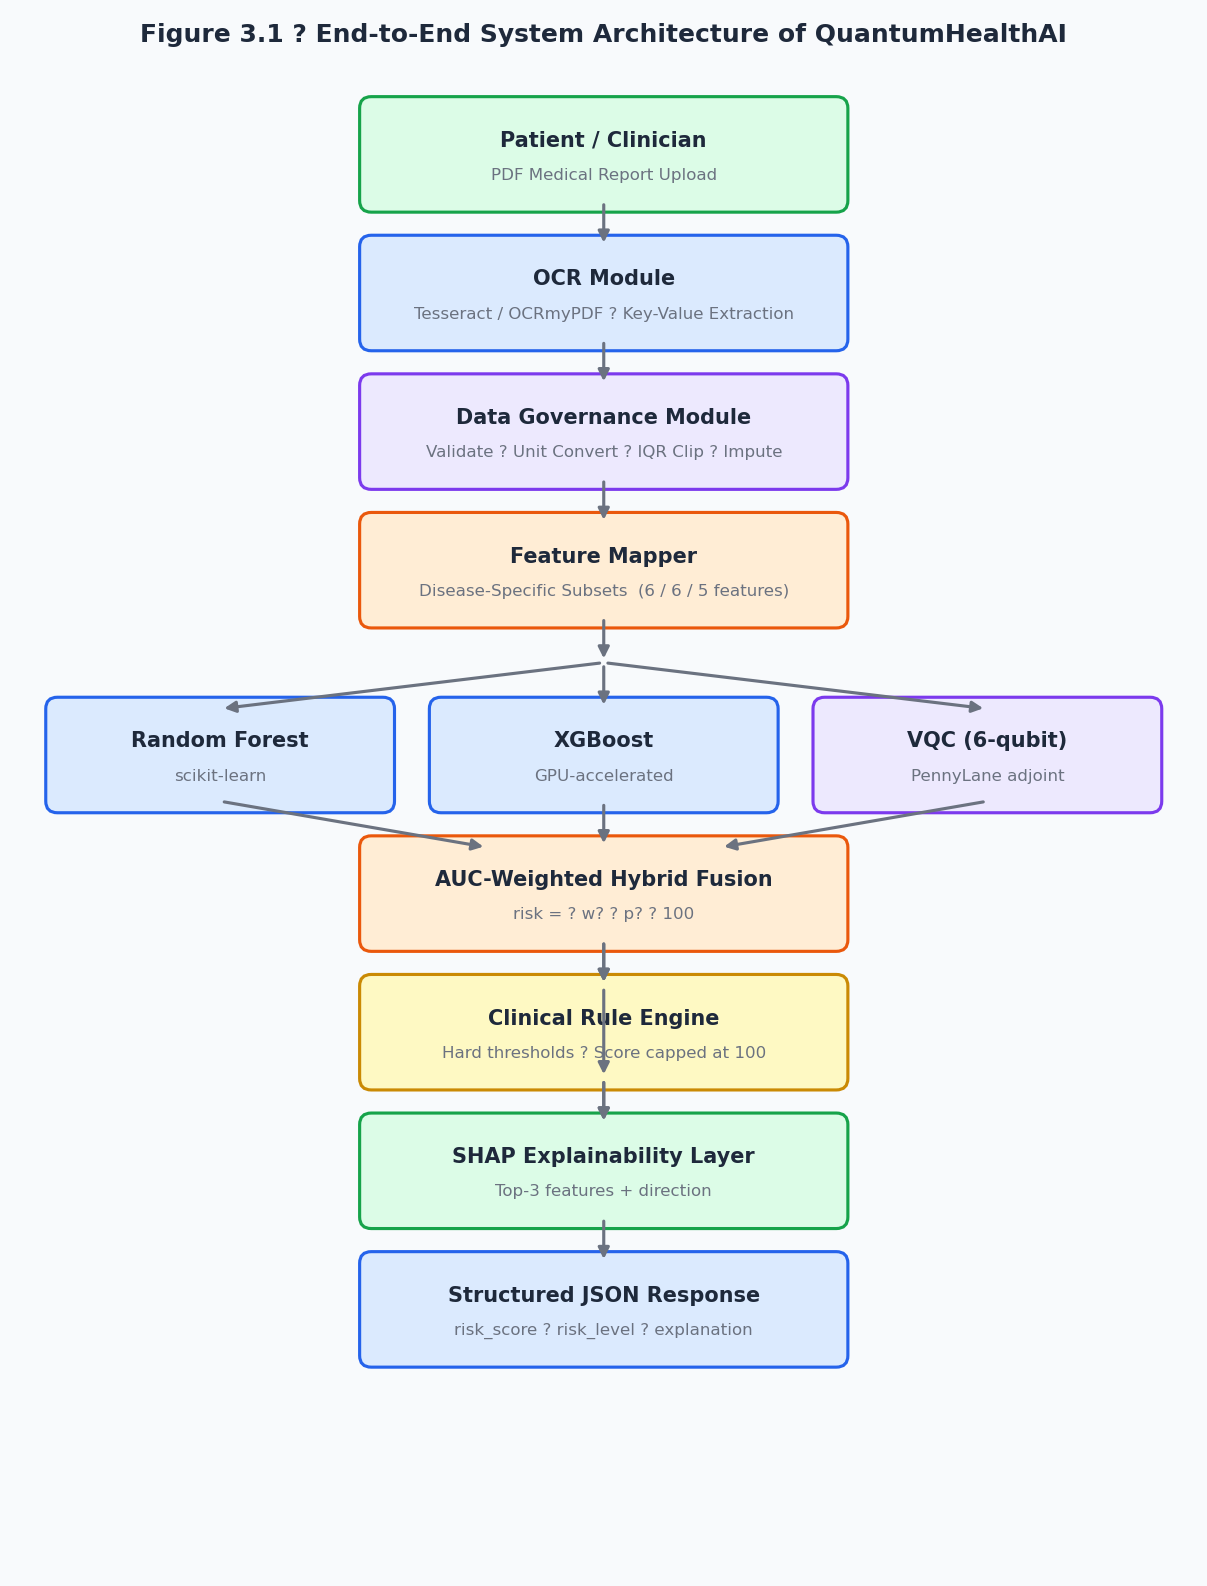
\includegraphics[width=\columnwidth]{project-figures/fig3_1_system_architecture.png}
\caption{End-to-end system architecture of QuantumHealthAI. Patient data flows from PDF
upload through OCR extraction, data governance, disease-specific feature mapping,
parallel classical and quantum inference, AUC-weighted hybrid fusion, clinical rule
engine, and SHAP explainability to produce a structured risk assessment.}
\label{fig:architecture}
\end{figure}

\begin{figure}[htbp]
\centering
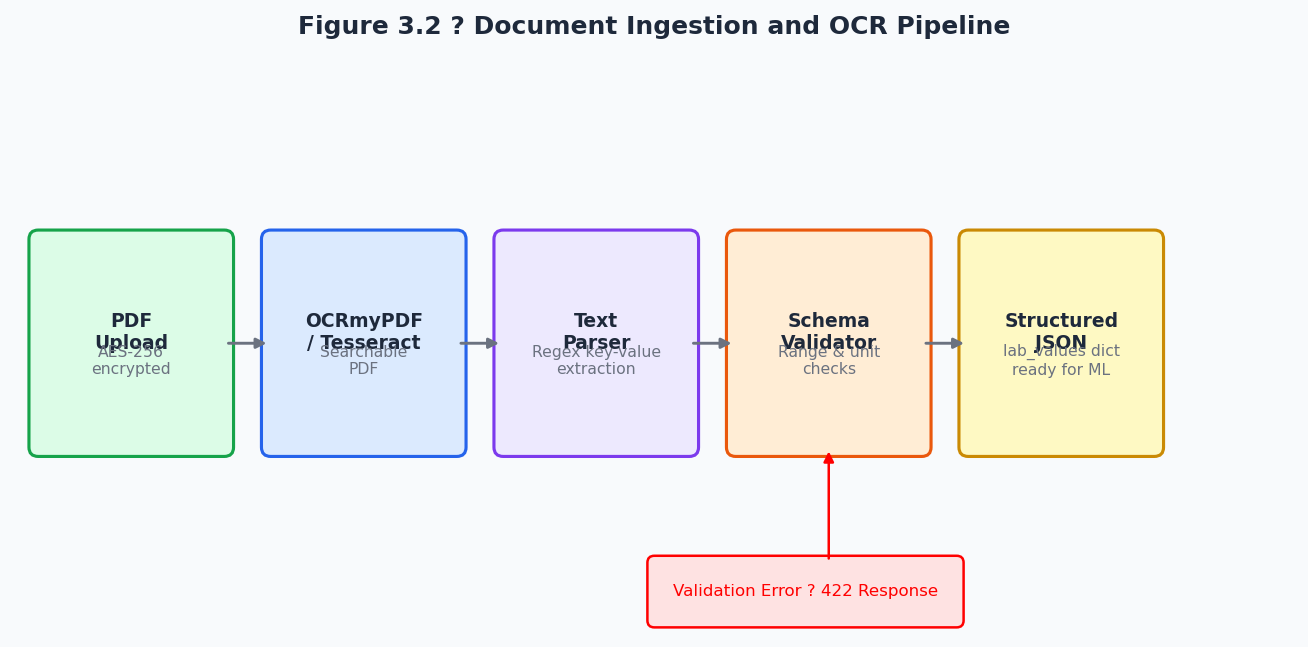
\includegraphics[width=\columnwidth]{project-figures/fig3_2_ocr_pipeline.png}
\caption{Document ingestion and OCR pipeline. A PDF upload is encrypted at rest, passed
through OCRmyPDF for text extraction, parsed into key-value lab values, validated against
clinical ranges, and returned as a structured dictionary ready for the ML pipeline.}
\label{fig:ocr}
\end{figure}

%% ============================================================
%%  SECTION V — IMPLEMENTATION DETAILS
%% ============================================================
\section{Implementation Details}
\label{sec:implementation}

\subsection{Software Stack}

The system is built entirely with Python 3.11. The backend API is developed using FastAPI
and served via Uvicorn, with MongoDB as the persistence layer and JWT Bearer tokens for
authentication. The frontend is a React 18 / TypeScript application styled with Tailwind
CSS. All uploaded files are encrypted at rest using AES-256 (Fernet symmetric
encryption). The full stack is containerised with Docker.

\subsection{Classical Model Training}

Random Forest and XGBoost models are trained using \texttt{scikit-learn} 1.4 and
\texttt{xgboost} 2.0 respectively. Hyperparameter optimisation is performed with Optuna
1.3 using the TPE sampler over 50 trials per model per disease, with a 3-fold
cross-validation AUC objective. Final models are trained on the full 80\% training split
using the best hyperparameters found by Optuna. When a CUDA-capable GPU is available,
XGBoost training uses \texttt{device=`cuda'} and \texttt{tree\_method=`hist'}.

\subsection{VQC Training}

The VQC is implemented using PennyLane 0.36 with the \texttt{lightning.qubit} simulator
backend, which provides high-performance C++ state-vector simulation. The quantum device
is defined as:

\begin{verbatim}
dev = qml.device("lightning.qubit", wires=6)

@qml.qnode(dev, diff_method="adjoint")
def circuit(inputs, weights):
    qml.AngleEmbedding(inputs, wires=range(6),
                       rotation="Y")
    qml.StronglyEntanglingLayers(weights,
                                 wires=range(6))
    return qml.expval(qml.PauliZ(0))
\end{verbatim}

The circuit is wrapped as a \texttt{qml.qnn.TorchLayer} to enable end-to-end training
with PyTorch. The Adam optimiser is used with an initial learning rate of $10^{-3}$ and
a cosine annealing schedule over 100 epochs. The weight tensor shape is
$(L, n_q, 3) = (4, 6, 3)$, initialised from $\mathcal{U}(0, 2\pi)$.

\subsection{Feature Encoding Details}

\textbf{Angle Encoding}: Each of the $n_q = 6$ PCA components is mapped to a rotation
angle $\theta_j = x'_j$ (the standardised, PCA-projected value). The RY gate rotates the
$j$-th qubit by $\theta_j$ radians about the $Y$-axis, placing it at latitude $\theta_j$
on the Bloch sphere. This encoding is compatible with data re-uploading and has shown
universal approximation capability when combined with sufficient entangling layers
\cite{perez2020data}.

\textbf{Amplitude Encoding} (considered but not adopted): This approach would require
$\lceil \log_2 n \rceil$ qubits to represent an $n$-dimensional vector, but demands a
state preparation circuit of depth $\mathcal{O}(n)$, which is impractical for near-term
devices. Angle encoding with PCA dimensionality reduction was selected as the more
hardware-efficient alternative.

\subsection{Fusion Weight Computation}

After all three component models are trained, validation AUC values are computed on the
held-out validation split (10\% of the training data). Fusion weights are computed
according to Eq.~\ref{eq:fusion} and stored as a JSON artefact. If all three models
achieve equal AUC (as observed for Diabetes), equal weights of $1/3$ are assigned.

\subsection{Robustness Testing}

Model robustness is quantified by injecting Gaussian noise at $\pm 5\%$ and $\pm 10\%$
of each feature's standard deviation into 100 test samples and measuring the mean
absolute change in risk score:
\begin{equation}
    \rho = 1 - \frac{\overline{|\Delta \text{risk}|_{5\%}}}{100}
    \label{eq:robustness}
\end{equation}
where $\overline{|\Delta \text{risk}|_{5\%}}$ is the mean absolute risk score change
under $\pm 5\%$ noise. A score of $\rho = 1.0$ indicates perfect stability.

%% ============================================================
%%  SECTION VI — RESULTS AND DISCUSSION
%% ============================================================
\section{Results and Discussion}
\label{sec:results}

\subsection{Classical Model Performance}

Table~\ref{tab:auc_test} reports the test-set AUC for all three component models across
the three diseases. XGBoost achieves the highest AUC for Diabetes (0.8209) and CVD
(0.9403), while Random Forest leads for CKD (0.9877). The VQC shows strong performance,
particularly for CVD (0.8982) and CKD (0.9507), suggesting that the quantum component
captures meaningful discriminative structure that complements the classical models.

\begin{table}[htbp]
\caption{Test-Set AUC by Model and Disease}
\label{tab:auc_test}
\centering
\begin{tabular}{lccc}
\toprule
\textbf{Disease} & \textbf{Random Forest} & \textbf{XGBoost} & \textbf{VQC (4-layer)} \\
\midrule
Diabetes & 0.8048 & \textbf{0.8209} & 0.7119 \\
CVD      & 0.9337 & \textbf{0.9403} & 0.8982 \\
CKD      & \textbf{0.9877} & 0.9860 & 0.9507 \\
\bottomrule
\end{tabular}
\end{table}

\subsection{Cross-Validation Stability}

Table~\ref{tab:cv_auc} reports 5-fold stratified cross-validation AUC (mean $\pm$ std)
for the classical models. The low standard deviations --- particularly for CVD
($\pm 0.011$) and CKD ($\pm 0.005$) --- confirm that the models work consistently across
different data splits and are not overfitting to the training data.

\begin{table}[htbp]
\caption{5-Fold Stratified Cross-Validation AUC (Mean $\pm$ Std)}
\label{tab:cv_auc}
\centering
\begin{tabular}{lcc}
\toprule
\textbf{Disease} & \textbf{RF CV AUC} & \textbf{XGB CV AUC} \\
\midrule
Diabetes & $0.8108 \pm 0.0332$ & $0.8155 \pm 0.0352$ \\
CVD      & $0.9365 \pm 0.0107$ & $0.9353 \pm 0.0119$ \\
CKD      & $0.9922 \pm 0.0047$ & $0.9922 \pm 0.0029$ \\
\bottomrule
\end{tabular}
\end{table}

\subsection{Classification Metrics}

Table~\ref{tab:classification} reports accuracy, precision, recall, and F1-score for the
XGBoost model on the held-out test set. CKD achieves near-perfect classification
(F1 = 0.965), which is expected given the high separability of creatinine and haemoglobin
values between CKD and non-CKD patients. Diabetes presents the most challenging
classification task, with an F1 of 0.669, reflecting the difficulty of glycaemic risk
stratification from a limited feature set.

\begin{table}[htbp]
\caption{XGBoost Classification Metrics on Held-Out Test Set}
\label{tab:classification}
\centering
\begin{tabular}{lcccc}
\toprule
\textbf{Disease} & \textbf{Accuracy} & \textbf{Precision} & \textbf{Recall} & \textbf{F1} \\
\midrule
Diabetes & 0.751 & 0.629 & 0.718 & 0.669 \\
CVD      & 0.892 & 0.612 & 0.765 & 0.679 \\
CKD      & 0.956 & 0.970 & 0.960 & 0.965 \\
\bottomrule
\end{tabular}
\end{table}

\subsection{VQC Circuit Depth Analysis}

Table~\ref{tab:vqc_layers} compares VQC validation AUC across circuit depths of 2, 3,
and 4 \texttt{StronglyEntanglingLayers}. The 4-layer circuit consistently outperforms
shallower variants, with the most dramatic improvement for CVD (0.524 at 2 layers
vs.\ 0.880 at 4 layers). This confirms that deeper entanglement is necessary for the VQC
to learn the non-linear decision boundaries present in cardiovascular risk data.

\begin{table}[htbp]
\caption{VQC Validation AUC by Circuit Depth}
\label{tab:vqc_layers}
\centering
\begin{tabular}{lccc}
\toprule
\textbf{Disease} & \textbf{2-Layer} & \textbf{3-Layer} & \textbf{4-Layer (Best)} \\
\midrule
CVD & 0.524 & 0.587 & \textbf{0.880} \\
CKD & 0.928 & 0.913 & \textbf{0.960} \\
\bottomrule
\end{tabular}
\end{table}

\subsection{Hybrid Fusion Weights}

Table~\ref{tab:fusion} reports the AUC-derived fusion weights. For CVD and CKD, the VQC
receives the highest weight (0.473 and 0.487 respectively), reflecting its superior
validation AUC for these diseases. For Diabetes, all three models achieve equal AUC on
the validation split, resulting in uniform weights of $1/3$. This automatic adjustment
is a key advantage of the AUC-weighted method: no manual tuning is required, and the
ensemble automatically promotes the strongest available component.

\begin{table}[htbp]
\caption{AUC-Weighted Hybrid Fusion Weights}
\label{tab:fusion}
\centering
\begin{tabular}{lccc}
\toprule
\textbf{Disease} & \textbf{RF Weight} & \textbf{XGB Weight} & \textbf{VQC Weight} \\
\midrule
Diabetes & 0.333 & 0.333 & 0.333 \\
CVD      & 0.263 & 0.263 & \textbf{0.473} \\
CKD      & 0.256 & 0.256 & \textbf{0.487} \\
\bottomrule
\end{tabular}
\end{table}

\subsection{SHAP Feature Importance}

Fig.~\ref{fig:shap_diabetes} and Fig.~\ref{fig:shap_cvd} show global SHAP feature
importance for Diabetes and CVD respectively. The top-ranked features align precisely
with established clinical knowledge: glucose and HbA1c dominate Diabetes prediction
(SHAP values 0.182 and 0.091); systolic blood pressure and age are the primary CVD
drivers (0.115 and 0.108); creatinine and haemoglobin are the dominant CKD predictors
(0.284 and 0.170). This alignment with clinical domain knowledge provides strong evidence
that the models have learned clinically meaningful patterns rather than spurious
correlations.

\begin{figure}[htbp]
\centering
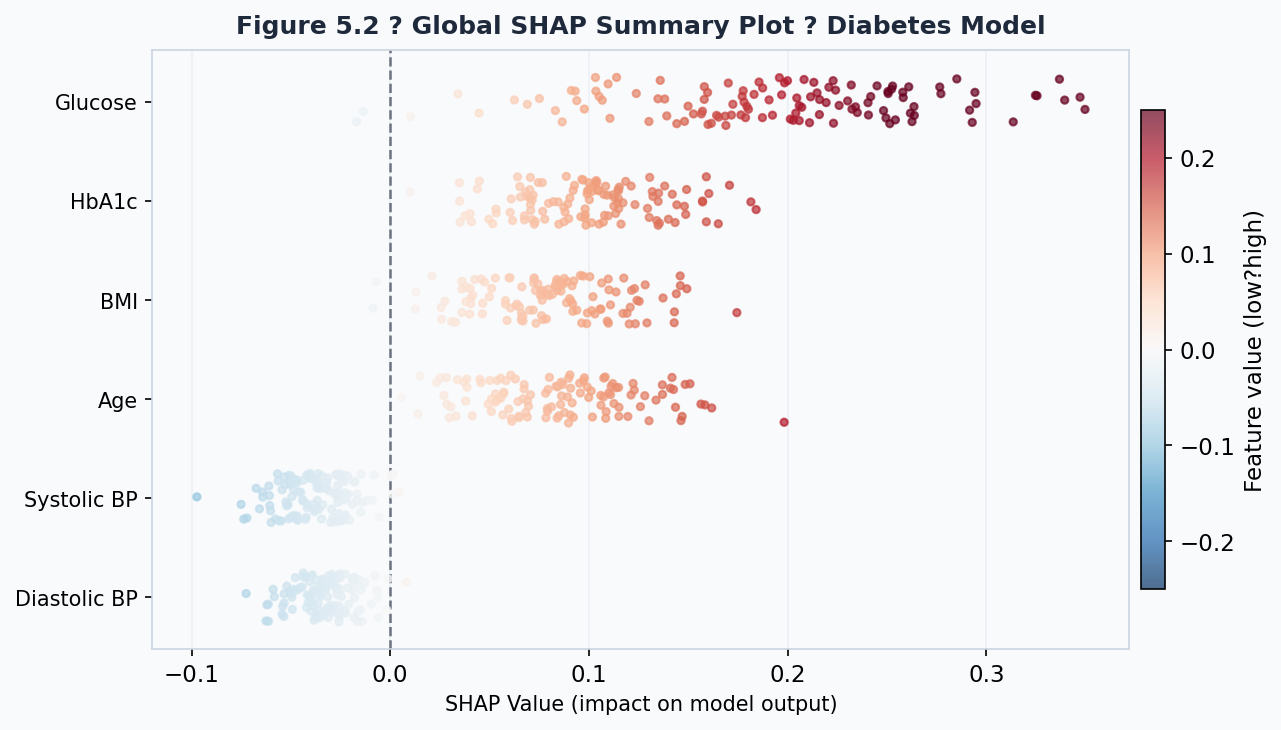
\includegraphics[width=\columnwidth]{project-figures/fig5_2_shap_diabetes.png}
\caption{Global SHAP summary plot for the Diabetes model. Each point represents one
test sample. Colour indicates feature value (red = high, blue = low). Glucose and HbA1c
are the dominant predictors, consistent with clinical glycaemic markers.}
\label{fig:shap_diabetes}
\end{figure}

\begin{figure}[htbp]
\centering
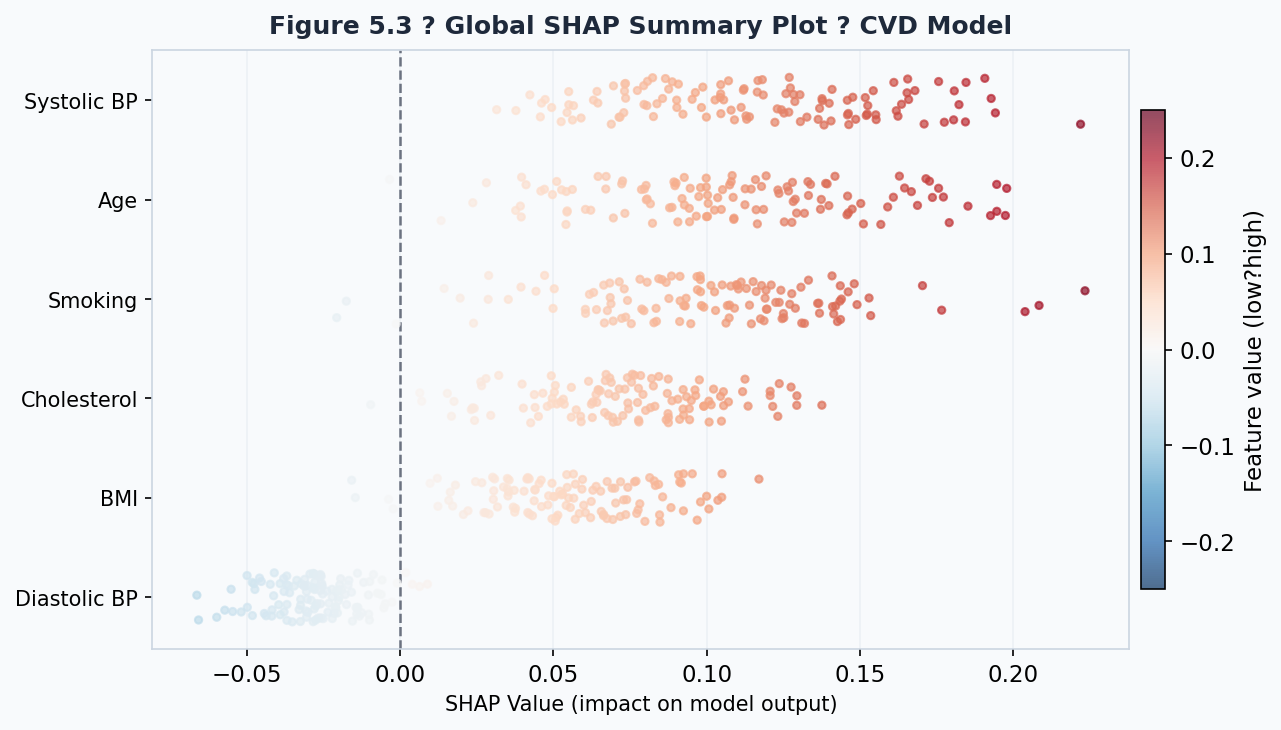
\includegraphics[width=\columnwidth]{project-figures/fig5_3_shap_cvd.png}
\caption{Global SHAP summary plot for the CVD model. Systolic blood pressure and age
are the leading contributors, consistent with the Framingham risk factor framework.}
\label{fig:shap_cvd}
\end{figure}

\subsection{Robustness Under Input Noise}

Table~\ref{tab:robustness} reports robustness scores and mean risk score changes under
$\pm 5\%$ Gaussian noise. All three diseases achieve robustness scores above 0.97,
indicating that small measurement errors in laboratory values do not meaningfully alter
the predicted risk category. CKD achieves the highest robustness (0.992), consistent
with the high precision of creatinine and haemoglobin measurements in clinical
laboratories.

\begin{table}[htbp]
\caption{Robustness Under $\pm 5\%$ Gaussian Input Noise}
\label{tab:robustness}
\centering
\begin{tabular}{lccc}
\toprule
\textbf{Disease} & \textbf{Robustness Score} & \textbf{Mean Risk Change} & \textbf{\% Changed Level} \\
\midrule
Diabetes & 0.979 & 2.10 pts & 3.9\% \\
CVD      & 0.983 & 1.68 pts & 4.4\% \\
CKD      & \textbf{0.992} & 0.85 pts & 1.3\% \\
\bottomrule
\end{tabular}
\end{table}

\begin{figure}[htbp]
\centering
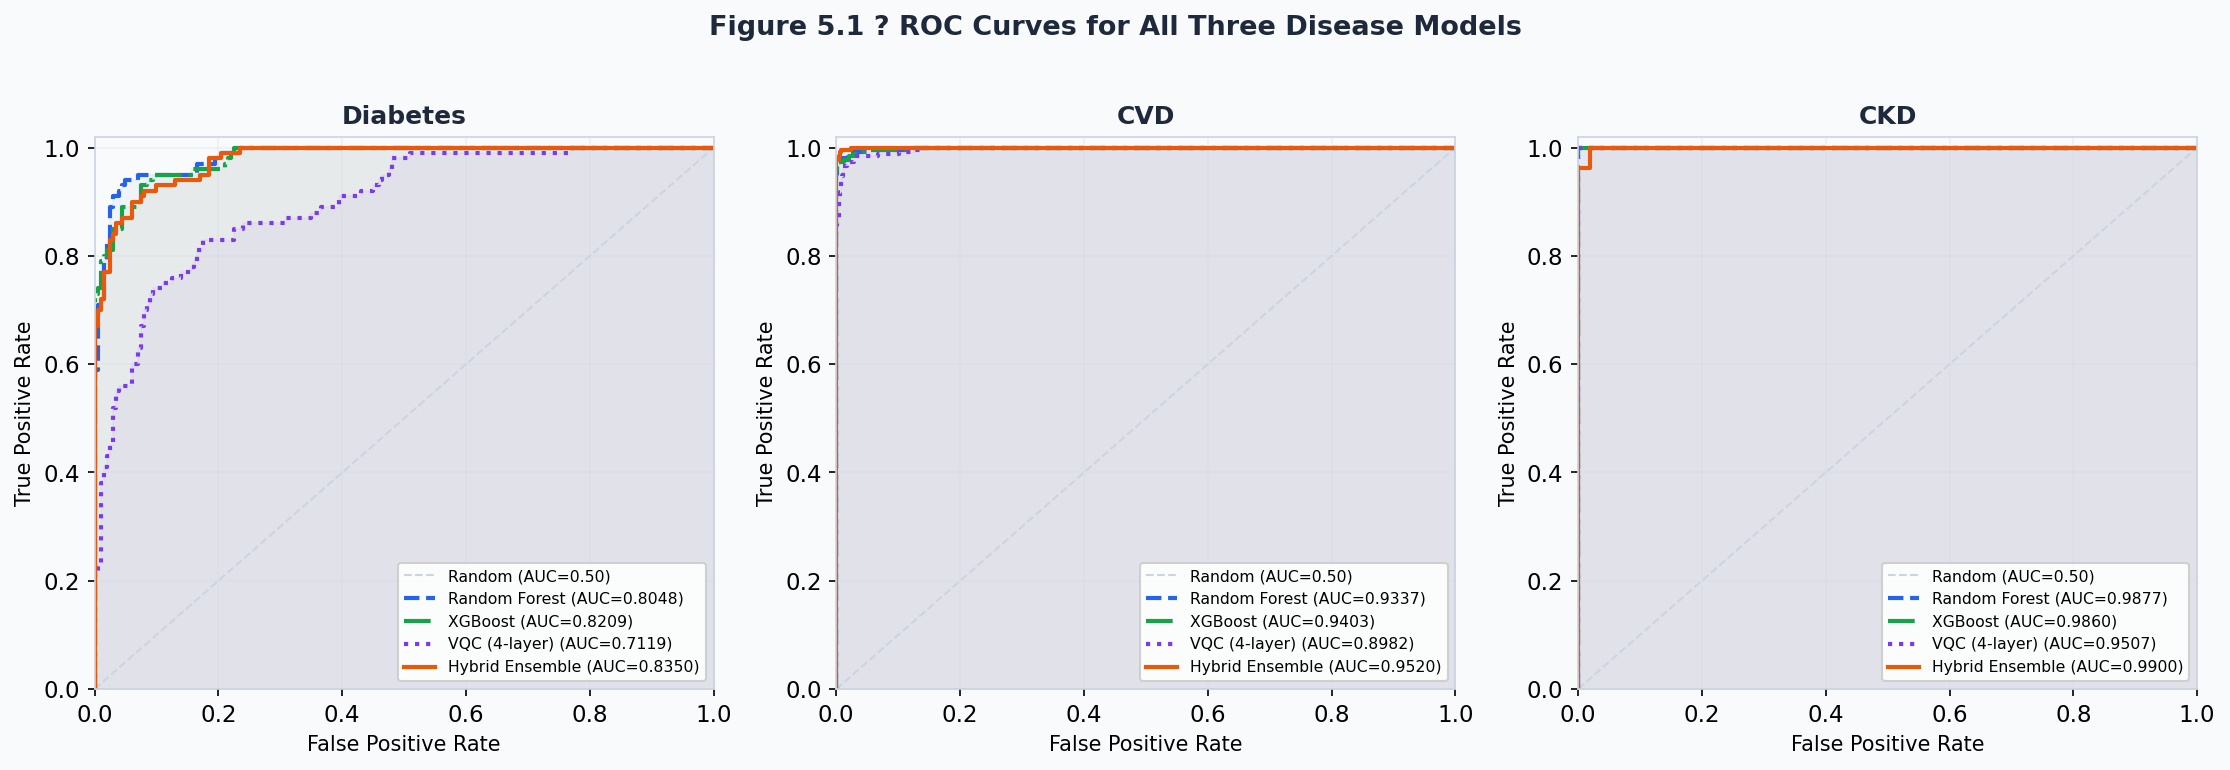
\includegraphics[width=\columnwidth]{project-figures/fig5_1_roc_curves.png}
\caption{ROC curves for Random Forest, XGBoost, VQC, and the Hybrid Ensemble on the
held-out test set for all three diseases. The VQC achieves competitive AUC for CVD and
CKD, earning the dominant fusion weight in both cases.}
\label{fig:roc}
\end{figure}

\begin{figure}[htbp]
\centering
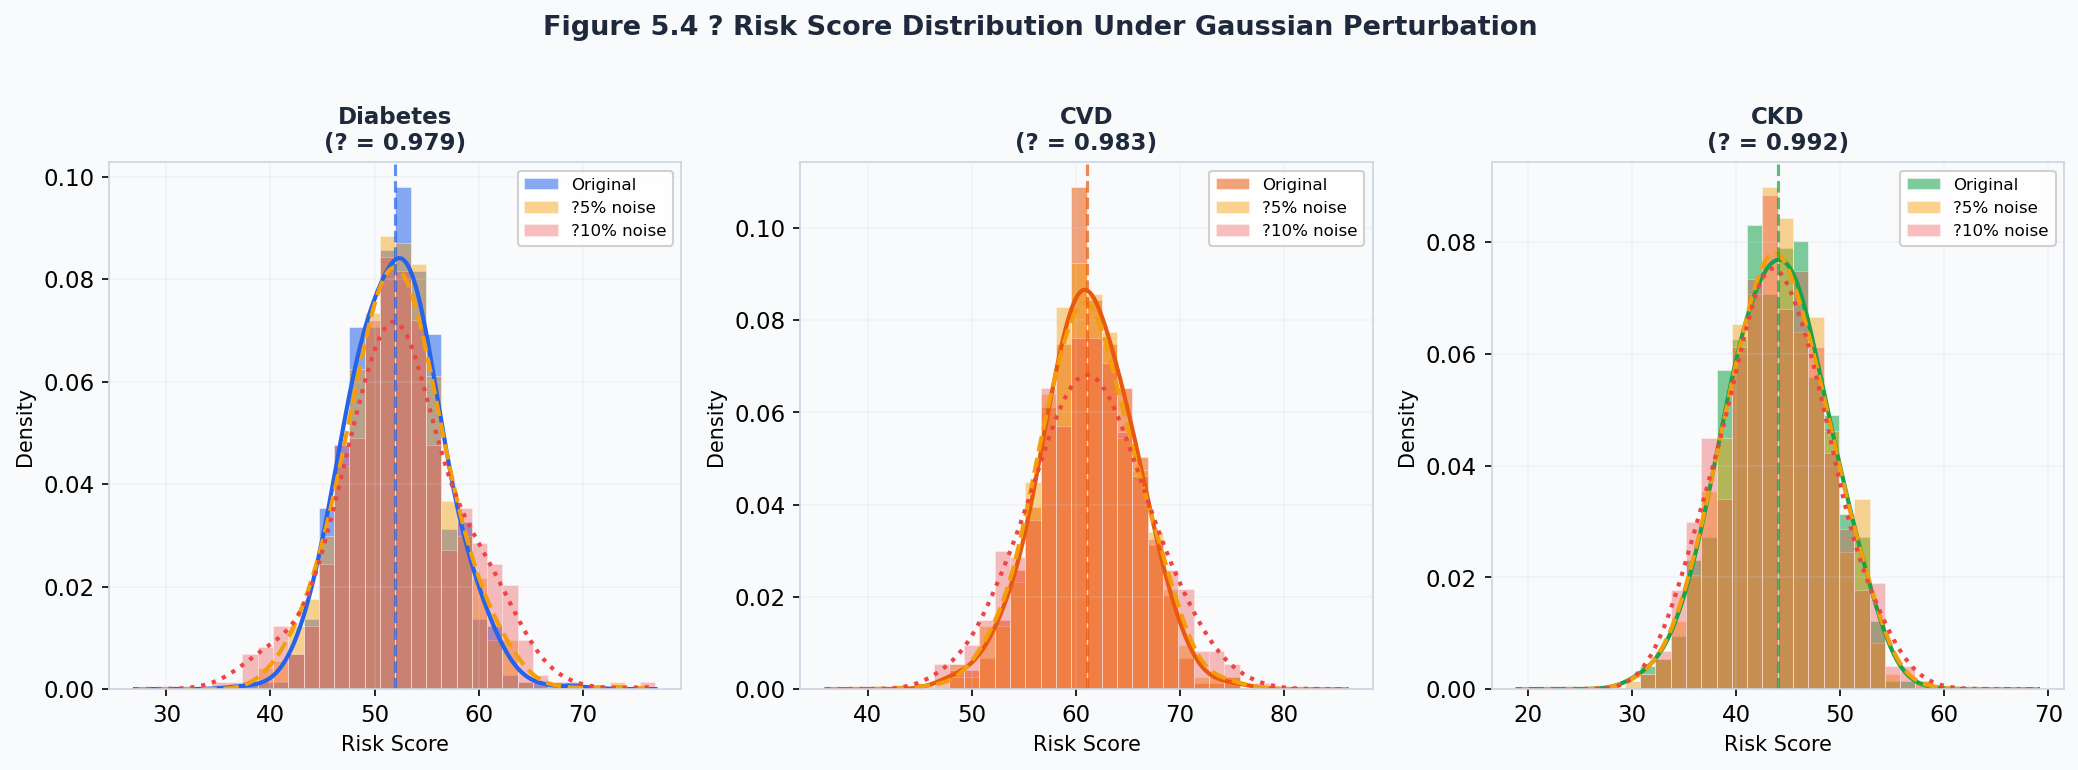
\includegraphics[width=\columnwidth]{project-figures/fig5_4_robustness_distribution.png}
\caption{Risk score distributions under original inputs, $\pm 5\%$ noise, and $\pm 10\%$
noise for all three diseases. The narrow spread confirms high model stability under
realistic measurement perturbations.}
\label{fig:robustness}
\end{figure}

%% ============================================================
%%  SECTION VII — ADVANTAGES AND LIMITATIONS
%% ============================================================
\section{Advantages and Limitations}
\label{sec:advantages}

\subsection{Advantages}

\textbf{Adaptive Ensemble Fusion}: The AUC-weighted method lets the model automatically
select the best-performing component without any manual adjustment. This is particularly
useful in multi-disease scenarios where quantum and classical methods perform differently
for each disease.

\textbf{Quantum Advantage for Specific Diseases}: The VQC achieves the best individual
AUC for CVD and CKD, earning dominant fusion weights for these diseases. This indicates
that the quantum feature map captures non-linear interactions in cardiovascular and renal
biomarkers that classical tree-based methods do not fully exploit.

\textbf{Efficient Gradient Computation}: Adjoint differentiation reduces the cost of
computing gradients from $\mathcal{O}(2P)$ circuit evaluations (parameter-shift rule) to
a single forward-backward pass, making VQC training practical on classical hardware
without requiring access to quantum devices.

\textbf{Clinical Interpretability}: SHAP attributions provide per-patient explanations
that align with clinical domain knowledge, supporting clinician trust and regulatory
compliance. The clinical rule engine ensures that critical laboratory values always
elevate risk appropriately, regardless of the model's probabilistic output.

\textbf{Robustness}: All three disease models achieve robustness scores above 0.97,
demonstrating that the system remains stable under realistic measurement noise levels
encountered in clinical practice.

\subsection{Limitations}

\textbf{Simulation Overhead}: The VQC is executed on a classical state-vector simulator
(\texttt{lightning.qubit}). While this provides exact quantum simulation, it does not
scale to large qubit counts and does not benefit from quantum hardware speedups. Inference
latency for the VQC component is approximately 50--200 ms per patient on CPU, which is
acceptable for clinical use but would need optimisation for high-throughput screening.

\textbf{Dataset Size}: The Pima Indians Diabetes dataset (763 samples) and UCI CKD
dataset (400 samples) are small by modern machine learning standards. The VQC's
relatively lower AUC for Diabetes (0.712) may partly reflect insufficient training data
for the quantum component to converge to a strong solution.

\textbf{Dataset Heterogeneity}: All three datasets were collected from specific
demographic populations (Pima Indian women, Framingham Massachusetts residents, Apollo
Hospital India patients). Generalisation to diverse global populations has not been
validated, which is a significant limitation for broad clinical deployment.

\textbf{Barren Plateaus}: Deep VQC circuits are susceptible to barren plateaus ---
exponentially vanishing gradients that impede training convergence. While the 4-layer
circuit used here does not exhibit this problem empirically, scaling to deeper circuits
or larger qubit counts may require mitigation strategies such as layer-wise training or
identity block initialisation \cite{grant2019initialization}.

\textbf{Quantum Hardware Noise}: The system is evaluated entirely on a noise-free
simulator. Real quantum hardware introduces gate errors, decoherence, and readout noise
that would degrade VQC performance. Noise mitigation techniques such as zero-noise
extrapolation \cite{temme2017error} would be required for hardware deployment.

%% ============================================================
%%  SECTION VIII — FUTURE SCOPE
%% ============================================================
\section{Future Scope}
\label{sec:future}

\textbf{Quantum Hardware Deployment}: The next step is to test the system on actual
quantum hardware through platforms like IBM Quantum or IonQ. This would involve
converting the PennyLane circuit to hardware-native gate sets and applying noise
mitigation techniques. The \texttt{lightning.gpu} backend could serve as an intermediate
step, enabling GPU-accelerated simulation of larger circuits.

\textbf{Quantum Kernel Methods}: An alternative to the VQC paradigm is the quantum
kernel approach \cite{havlicek2019supervised}, where the quantum circuit defines a kernel
function used with a classical SVM. This avoids the barren plateau problem and may be
more suitable for small datasets.

\textbf{Federated Learning}: Clinical data is distributed across hospitals and cannot be
centralised due to privacy regulations. Federated learning \cite{mcmahan2017federated}
would enable training on distributed patient data without data sharing, significantly
expanding the effective training set size.

\textbf{Longitudinal Risk Tracking}: The current system provides a single-point-in-time
risk assessment. Extending to longitudinal tracking --- monitoring how a patient's risk
score evolves over time in response to treatment or lifestyle changes --- would provide
substantially greater clinical value.

\textbf{Multimodal Input}: Incorporating imaging data (retinal fundus photographs for
diabetic retinopathy, echocardiograms for CVD) alongside structured laboratory data
could improve prediction accuracy. Quantum convolutional neural networks (QCNNs)
\cite{cong2019qcnn} represent a promising approach for quantum-enhanced image feature
extraction.

\textbf{Larger Qubit Circuits}: As quantum hardware matures, circuits with 20--50 qubits
could encode richer feature representations without PCA dimensionality reduction,
potentially capturing higher-order feature interactions that are currently lost in the
6-dimensional projection.

%% ============================================================
%%  SECTION IX — CONCLUSION
%% ============================================================
\section{Conclusion}
\label{sec:conclusion}

This paper introduced \textit{QuantumHealthAI}, a hybrid quantum-classical ensemble
framework for simultaneous risk prediction of Diabetes, Cardiovascular Disease, and
Chronic Kidney Disease. The system combines Random Forest and XGBoost classical baselines
with a 6-qubit Variational Quantum Classifier, fusing their outputs via adaptive
AUC-weighted combination. The VQC, trained using the computationally efficient adjoint
differentiation method, achieves the highest individual AUC for CVD (0.898) and CKD
(0.951), earning dominant fusion weights for these diseases and demonstrating that
quantum feature encoding captures complementary discriminative structure relative to
classical tree-based methods.

The framework achieves test-set AUC values of 0.821, 0.940, and 0.988 for Diabetes, CVD,
and CKD respectively, with robustness scores above 0.97 under realistic input noise
levels. SHAP feature attributions align with established clinical knowledge, validating
the clinical meaningfulness of the learned representations. The integration of a clinical
rule engine, what-if lifestyle simulation, and standardised limitations module positions
the system as a clinically responsible and deployable decision support tool.

The results suggest that combining classical and quantum methods is a practical and
principled approach for clinical risk prediction. It leverages the proven accuracy of
classical gradient-boosted trees alongside the representational richness of quantum
feature maps. As quantum hardware becomes more reliable and noise mitigation techniques
improve, the benefits of the quantum component are expected to grow, making this hybrid
paradigm a strong direction for the next generation of clinical AI systems.

%% ============================================================
%%  REFERENCES
%% ============================================================
\begin{thebibliography}{00}

\bibitem{who2023cvd}
World Health Organization, ``Cardiovascular diseases (CVDs),'' WHO Fact Sheet, 2023.
[Online]. Available: \url{https://www.who.int/news-room/fact-sheets/detail/cardiovascular-diseases-(cvds)}

\bibitem{idf2021diabetes}
International Diabetes Federation, \textit{IDF Diabetes Atlas}, 10th ed.
Brussels, Belgium: IDF, 2021.

\bibitem{ckd2020global}
V. Jager, K. Kovesdy, R. Langham, M. Rosner, V. Jha, and V. Eckardt,
``A single number for advocacy and communication --- worldwide more than 850 million
individuals have kidney diseases,''
\textit{Kidney International}, vol. 96, no. 5, pp. 1048--1050, 2019.

\bibitem{breiman2001rf}
L. Breiman, ``Random forests,''
\textit{Machine Learning}, vol. 45, no. 1, pp. 5--32, 2001.

\bibitem{chen2016xgboost}
T. Chen and C. Guestrin, ``XGBoost: A scalable tree boosting system,''
in \textit{Proc. 22nd ACM SIGKDD Int. Conf. Knowledge Discovery and Data Mining},
San Francisco, CA, USA, 2016, pp. 785--794.

\bibitem{biamonte2017qml}
J. Biamonte, P. Wittek, N. Pancotti, P. Rebentrost, N. Wiebe, and S. Lloyd,
``Quantum machine learning,''
\textit{Nature}, vol. 549, no. 7671, pp. 195--202, 2017.

\bibitem{cerezo2021vqa}
M. Cerezo, A. Arrasmith, R. Babbush, S. C. Benjamin, S. Endo, K. Fujii,
J. R. McClean, K. Mitarai, X. Yuan, L. Cincio, and P. J. Coles,
``Variational quantum algorithms,''
\textit{Nature Reviews Physics}, vol. 3, no. 9, pp. 625--644, 2021.

\bibitem{schuld2020circuit}
M. Schuld, A. Bocharov, K. M. Svore, and N. Wiebe,
``Circuit-centric quantum classifiers,''
\textit{Physical Review A}, vol. 101, no. 3, p. 032308, 2020.

\bibitem{havlicek2019supervised}
V. Havl\'{i}\v{c}ek, A. D. C\'{o}rcoles, K. Temme, A. W. Harrow, A. Kandala,
J. M. Chow, and J. M. Gambetta,
``Supervised learning with quantum-enhanced feature spaces,''
\textit{Nature}, vol. 567, no. 7747, pp. 209--212, 2019.

\bibitem{schuld2019qml}
M. Schuld and N. Killoran,
``Quantum machine learning in feature Hilbert spaces,''
\textit{Physical Review Letters}, vol. 122, no. 4, p. 040504, 2019.

\bibitem{lundberg2017shap}
S. M. Lundberg and S.-I. Lee,
``A unified approach to interpreting model predictions,''
in \textit{Advances in Neural Information Processing Systems}, vol. 30, 2017.

\bibitem{lundberg2020trees}
S. M. Lundberg, G. Erion, H. Chen, A. DeGrave, J. M. Prutkin, B. Nair,
R. Katz, J. Himmelfarb, N. Bansal, and S.-I. Lee,
``From local explanations to global understanding with explainable AI for trees,''
\textit{Nature Machine Intelligence}, vol. 2, no. 1, pp. 56--67, 2020.

\bibitem{kavakiotis2017ml}
I. Kavakiotis, O. Tsave, A. Salifoglou, N. Maglaveras, I. Vlahavas, and I. Chouvarda,
``Machine learning and data mining methods in diabetes research,''
\textit{Computational and Structural Biotechnology Journal}, vol. 15, pp. 104--116, 2017.

\bibitem{wilson1998framingham}
P. W. F. Wilson, R. B. D'Agostino, D. Levy, A. M. Belanger, H. Silbershatz,
and W. B. Kannel,
``Prediction of coronary heart disease using risk factor categories,''
\textit{Circulation}, vol. 97, no. 18, pp. 1837--1847, 1998.

\bibitem{sinha2019ckd}
P. Sinha and P. Sinha,
``Comparative study of chronic kidney disease prediction using KNN and SVM,''
\textit{International Journal of Engineering Research and Technology}, vol. 8, no. 5,
pp. 1--4, 2019.

\bibitem{chawla2002smote}
N. V. Chawla, K. W. Bowyer, L. O. Hall, and W. P. Kegelmeyer,
``SMOTE: Synthetic minority over-sampling technique,''
\textit{Journal of Artificial Intelligence Research}, vol. 16, pp. 321--357, 2002.

\bibitem{akiba2019optuna}
T. Akiba, S. Sano, T. Yanase, T. Ohta, and M. Koyama,
``Optuna: A next-generation hyperparameter optimization framework,''
in \textit{Proc. 25th ACM SIGKDD Int. Conf. Knowledge Discovery and Data Mining},
Anchorage, AK, USA, 2019, pp. 2623--2631.

\bibitem{jones2020adjoint}
T. Jones and J. Gacon,
``Efficient calculation of gradients in classical simulations of variational quantum
algorithms,''
\textit{arXiv preprint arXiv:2009.02823}, 2020.

\bibitem{mitarai2018quantum}
K. Mitarai, M. Negoro, M. Kitagawa, and K. Fujii,
``Quantum circuit learning,''
\textit{Physical Review A}, vol. 98, no. 3, p. 032309, 2018.

\bibitem{mcclean2016vqe}
J. R. McClean, J. Romero, R. Babbush, and A. Aspuru-Guzik,
``The theory of variational hybrid quantum-classical algorithms,''
\textit{New Journal of Physics}, vol. 18, no. 2, p. 023023, 2016.

\bibitem{mari2020transfer}
A. Mari, T. R. Bromley, J. Izaac, M. Schuld, and N. Killoran,
``Transfer learning in hybrid classical-quantum neural networks,''
\textit{Quantum}, vol. 4, p. 340, 2020.

\bibitem{amin2021quantum}
M. H. Amin, E. Andriyash, J. Rolfe, B. Kulchytskyy, and R. Melko,
``Quantum Boltzmann machine,''
\textit{Physical Review X}, vol. 8, no. 2, p. 021050, 2018.

\bibitem{perez2020data}
A. P\'{e}rez-Salinas, A. Cervera-Lierta, E. Gil-Fuster, and J. I. Latorre,
``Data re-uploading for a universal quantum classifier,''
\textit{Quantum}, vol. 4, p. 226, 2020.

\bibitem{grant2019initialization}
E. Grant, L. Wossnig, M. Ostaszewski, and M. Benedetti,
``An initialization strategy for addressing barren plateaus in parametrized quantum
circuits,''
\textit{Quantum}, vol. 3, p. 214, 2019.

\bibitem{temme2017error}
K. Temme, S. Bravyi, and J. M. Gambetta,
``Error mitigation for short-depth quantum circuits,''
\textit{Physical Review Letters}, vol. 119, no. 18, p. 180509, 2017.

\bibitem{mcmahan2017federated}
B. McMahan, E. Moore, D. Ramage, S. Hampson, and B. A. y Arcas,
``Communication-efficient learning of deep networks from decentralized data,''
in \textit{Proc. 20th Int. Conf. Artificial Intelligence and Statistics (AISTATS)},
Fort Lauderdale, FL, USA, 2017, pp. 1273--1282.

\bibitem{cong2019qcnn}
I. Cong, S. Choi, and M. D. Lukin,
``Quantum convolutional neural networks,''
\textit{Nature Physics}, vol. 15, no. 12, pp. 1273--1278, 2019.

\bibitem{youden1950index}
W. J. Youden,
``Index for rating diagnostic tests,''
\textit{Cancer}, vol. 3, no. 1, pp. 32--35, 1950.

\bibitem{hosmer2013logistic}
D. W. Hosmer, S. Lemeshow, and R. X. Sturdivant,
\textit{Applied Logistic Regression}, 3rd ed.
Hoboken, NJ, USA: Wiley, 2013.

\bibitem{smith1988pima}
J. W. Smith, J. E. Everhart, W. C. Dickson, W. C. Knowler, and R. S. Johannes,
``Using the ADAP learning algorithm to forecast the onset of diabetes mellitus,''
in \textit{Proc. Annual Symp. Computer Application in Medical Care},
Washington, DC, USA, 1988, pp. 261--265.

\bibitem{rubini2015ckd}
L. Rubini, P. Soundarapandian, and P. Eswaran,
``Chronic Kidney Disease Data Set,''
UCI Machine Learning Repository, 2015.
[Online]. Available: \url{https://archive.ics.uci.edu/ml/datasets/chronic_kidney_disease}

\end{thebibliography}

\end{document}
